\newpage
\section{Specifica del Back-End}
\subsection{QuizziPedia::Back-End}
\subsubsection{Informazioni generali}
\label{QuizziPedia::Back-End}
\begin{figure}
	\centering
	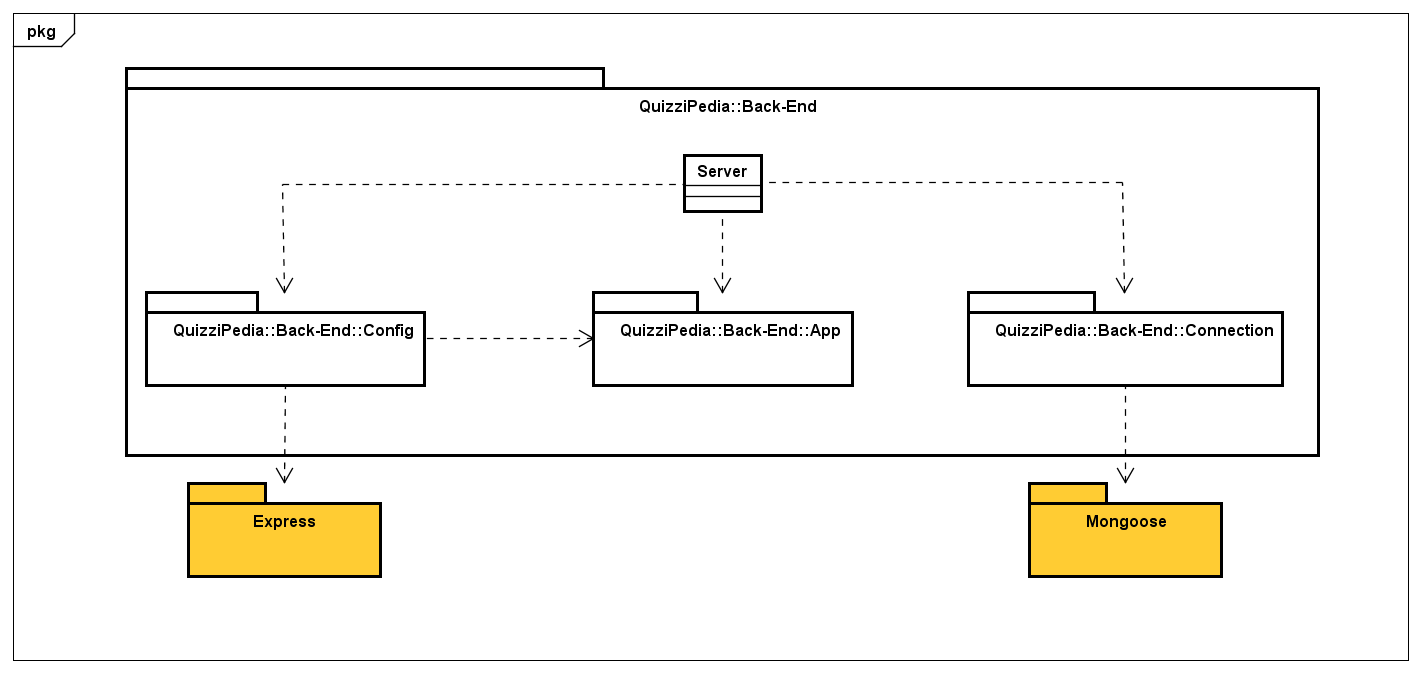
\includegraphics[scale=0.45]{UML/Package/QuizziPedia_Back-End.png}
	\caption{QuizziPedia::Back-End}
\end{figure}

	\begin{itemize}
		\item \textbf{Descrizione} \\ Package contenenti le componenti della parte back-end dell' applicazione.
		\item \textbf{Package contenuti}
		\begin{itemize}
			\item App \\
			Package\ped{G} contenente le componenti del server che implementano il \textit{pattern MVC\ped{G}}.
			\item Config \\
			Package\ped{G} contenente le componenti di configurazione del server\ped{G}.
		\end{itemize}
	\end{itemize}
\subsubsection{Classi}
	\paragraph{QuizziPedia::Back-End::Server}
	\begin{itemize}
		\item \textbf{Descrizione}
		\item \textbf{Utilizzo}
		\item \textbf{Relazioni con altre classi}
		\item \textbf{Attributi}
		\item \textbf{Metodi}
	\end{itemize}

\subsection{QuizziPedia::Back-End::Connection}
\subsubsection{Informazioni generali}
\subsubsection{Classi}

\subsection{QuizziPedia::Back-End::App}
\subsubsection{Informazioni generali}
\label{QuizziPedia::Back-End::App}
\begin{figure}
	\centering
	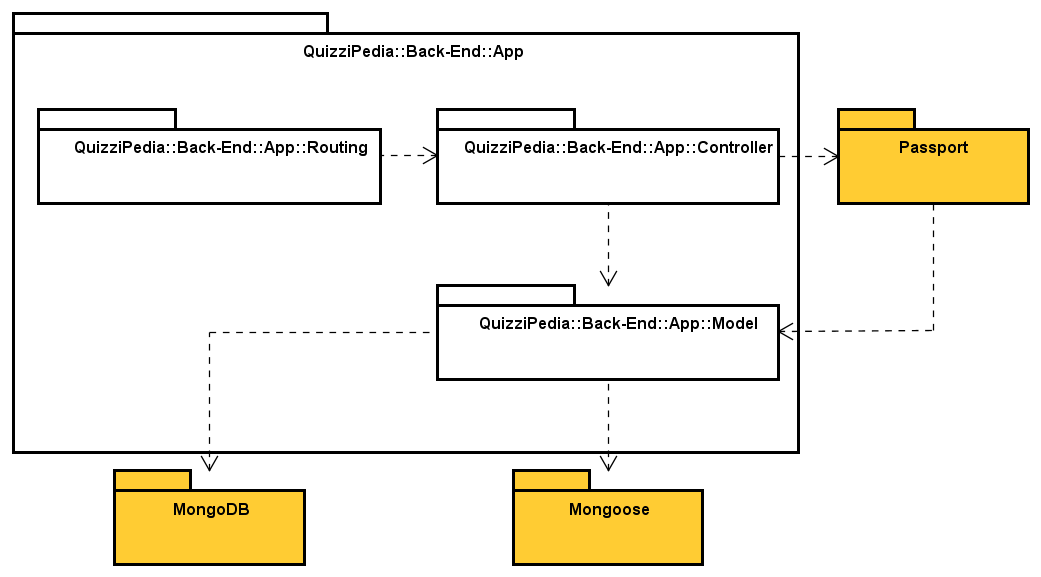
\includegraphics[scale=0.45]{UML/Package/QuizziPedia_Back-End_App.png}
	\caption{QuizziPedia::Back-End::App}
\end{figure}
	\begin{itemize}
		\item \textbf{Descrizione} \\
		Package contenente le componenti del server che implementano il \textit{pattern\ped{G} MVC\ped{G}};
		\item \textbf{Padre} \\ Back-End;
		\item \textbf{Interazioni con altri componenti}
			\begin{itemize}
				\item Congif \\
				Package contenente le componenti di configurazione del server;
			\end{itemize}
		\item \textbf{Package contenuti}
			\begin{itemize}
				\item Controllers \\
				Package che contiene i controllers di Express, definisce la logica dell'applicazione;
				\item Models \\
				Package che contiene le classi che definiscono il model dell'applicazione. Queste classi cono definite come classi schema di \textit{Mongoose\ped{G}}, il quale permette di utilizzare \textit{MongoDB\ped{G}} tramite degli oggetti;
				\item Routers \\
				Package contenente i routers della componente back-end dell'applicazione. Contiene i file di configurazione relativi al routing delle richieste del client, ossia i routers di Express.
			\end{itemize}
	\end{itemize}
	
\subsection{QuizziPedia::Back-End::App::Controllers}
\subsubsection{Informazioni generali}
	\begin{itemize}
		\item \textbf{Descrizione} \\
		\item \textbf{Padre} \\
		\item \textbf{Interazioni con altri componenti} \\
		\item \textbf{Package contenuti}
	\end{itemize}
\subsubsection{Classi}
\paragraph{QuizziPedia::Back-End::App::Controllers::NOMECLASSE}
	\begin{itemize}
		\item \textbf{Descrizione} \\
		\item \textbf{Utilizzo} \\
		\item \textbf{Relazioni con altre classi} \\
		\item \textbf{Metodi} \\
	\end{itemize}


\subsection{QuizziPedia::Back-End::App::Models}
\subsubsection{Informazioni generali}
\subsubsection{Classi}
\paragraph{QuizziPedia::Back-End::App::Models::NOMECLASSE}
\begin{itemize}
	\item \textbf{Descrizione} \\
	\item \textbf{Utilizzo} \\
	\item \textbf{Relazioni con altre classi} \\
	\item \textbf{Metodi} \\
\end{itemize}

\subsection{QuizziPedia::Back-End::App::Routers}
\subsubsection{Informazioni generali}
\subsubsection{classi}
\paragraph{QuizziPedia::Back-End::App::Routers::NOMECLASSE}
	\begin{itemize}
		\item \textbf{Descrizione} \\
		\item \textbf{Utilizzo} \\
		\item \textbf{Relazioni con altre classi} \\
		\item \textbf{Metodi} \\
<<<<<<< HEAD
	\end{itemize}
=======
	\end{itemize}
>>>>>>> origin/master
